\documentclass[11pt]{report} 
\usepackage{float}
\usepackage[a4paper, margin=0.9in]{geometry}
\usepackage{graphicx}
\usepackage{hyperref}
\usepackage{wrapfig}
\usepackage{acronym}
\usepackage{rotating}
\usepackage{glossaries}
\usepackage{mdframed}
\usepackage{enumitem}
\usepackage[table]{xcolor}
\usepackage[raster]{tcolorbox}
\usepackage{caption}
\usepackage[french]{babel}
\usepackage{setspace}  % Pour le contrôle de l'espacement des lignes
\usepackage[T1]{fontenc}
\usepackage{pgfgantt}

\definecolor{swotS}{RGB}{226,237,143}
\definecolor{swotW}{RGB}{247,193,139}
\definecolor{swotO}{RGB}{173,208,187}
\definecolor{swotT}{RGB}{192,165,184}

\usepackage{listings}
\lstset{
    basicstyle=\ttfamily\small,
    keywordstyle=\color{blue},
    commentstyle=\color{orange},
    stringstyle=\color{red},
    breaklines=true,
    numbers=left,
    numberstyle=\tiny\color{gray},
    frame=single,
    captionpos=b
}

\hypersetup{
    colorlinks=true,
    linkcolor=blue,
    filecolor=magenta,
    urlcolor=cyan,
    pdftitle={Rapport de Projet de Fin d'Année}
}

\begin{document}
\onehalfspacing  % Espacement d'une ligne et demie pour tout le document

% Page de garde
\begin{titlepage}

\begin{figure}[H]
    \centering
\begin{center}
\begin{minipage}{0.2\textwidth}
    \centering
    
\includegraphics[width=1.3\linewidth]{logo-ensa-berrechid.png}
\end{minipage}\hfill
\begin{minipage}{0.5\textwidth}
    \centering
    {\footnotesize \bf ROYAUME DU MAROC\\
    UNIVERSITÉ HASSAN PREMIER\\
    ÉCOLE NATIONALE DES SCIENCES APPLIQUÉES BERRECHID}
\end{minipage}\hfill
\begin{minipage}{0.1\textwidth}
    \centering
    
\includegraphics[width=1.3\linewidth]{uh1.png}
\end{minipage}
\end{center}
\end{figure}

\begin{center}
\vspace{2.5cm}

{\LARGE \textbf{Rapport de Projet de Fin d'Année}}\\[0.5cm]

{\large \textit{Spécialité : }\textbf{Ingénierie des Systèmes d'Information et Big Data}}\\[1.5cm]

\rule{\linewidth}{0.5mm}\\[0.4cm]
{\Large \textbf{AI Bio Profile Generator
}}\\[0.4cm]
\rule{\linewidth}{0.5mm}\\[0.5cm]

{\large Effectué à \textbf{SEGULA Technologies}}\\[0.5cm]
\begin{figure}[H]
    \centering
    
\includegraphics[width=0.45\linewidth]{chapters/SEGULA_Technologies_logo.png}
    
\end{figure} \\[2cm]

\begin{minipage}{0.45\textwidth}
    \begin{flushleft} \large
        \emph{Réalisé par :}\\
        \textbf{FARMATI Aya}
    \end{flushleft}
\end{minipage}
\begin{minipage}{0.45\textwidth}
    \begin{flushright} \large
        \emph{Encadré par :}\\
        \textbf{Mr. Hamza Moubariki      }\\
        \textbf{Mme. Fatima Ezzahra Saissi}
    \end{flushright}
\end{minipage}\\[2cm]

\vfill

{\large Soutenu le [Date], devant le jury :}\\[0.5cm]
\begin{center}
    Mr. [Nom du Membre 1]\\
    Mr. [Nom du Membre 2]
\end{center}

\vfill

{\large Année Universitaire : 2025-2026}
\end{center}
\end{titlepage}

\pagenumbering{roman}

\chapter*{Remerciements}
\addcontentsline{toc}{chapter}{Remerciements}
% remerciements.tex





{\itshape En clôture de cette étape importante de mon parcours académique et professionnel, il est essentiel pour
moi d’exprimer ma sincère gratitude et mes profonds remerciements à toutes les personnes qui ont joué un
rôle crucial dans la réalisation de mon projet de stage. Leur soutien, leurs conseils et leur présence ont été
des piliers de cette aventure.
\par\bigskip

Je tiens tout d’abord à exprimer ma reconnaissance au groupe \textbf{SEGULA Technologies} pour
m’avoir ouvert les portes de leur prestigieuse organisation. Grâce à eux, j’ai pu bénéficier d’un environne
ment de travail stimulant et propice à l’apprentissage, essentiel à l’accomplissement de mon projet.
\par\bigskip

Un merci tout particulier à \textbf{Monsieur MOUBARIKI Hamza}, mon encadrant  professionnel au sein
de \textbf{SEGULA Technologies}. Son accompagnement attentif, ses orientations précises et son expertise
ont grandement contribué à orienter mes efforts et à affiner mes compétences. Sa disponibilité exceptionnelle
et son soutien continu ont été des éléments déterminants de mon succès.
\par\bigskip

Je souhaite également remercier chaleureusement Madame \textbf{Fatima Ezzahra Saissi }, mon enseignante
et encadrante académique. Son encadrement rigoureux, ses conseils avisés et son encouragement constant ont
été des atouts inestimables tout au long de ce projet. Sa capacité à me guider dans la complexité des défis
rencontrés a été fondamentale pour mon croissance professionnelle et personnelle.
\par\bigskip

Je tiens aussi à remercier l’ensemble du personnel de SEGULA Technologies. Leur accueil, leur
disponibilité et leur aide ont contribué à créer une atmosphère de travail agréable et enrichissante, où l’apprentissage et le développement professionnel peuvent se dérouler dans les meilleures conditions.
\par\bigskip

Enfin, mes pensées les plus profondes vont à ma famille, mes proches et mes amis, qui ont fourni un
soutien émotionnel sans faille. Leur foi en mes capacités, leur écoute et leurs encouragements constants ont
été des sources de motivation indispensables. Je leur suis infiniment reconnaissant pour tout l’amour et le
soutien qu’ils m’ont témoignés durant cette période.

\par\bigskip
}



\chapter*{Résumé}
\addcontentsline{toc}{chapter}{Résumé}



Ce document constitue le rapport de mon stage de Projet de Fin d'Année (PFA), d'une durée de 2 mois. Cette expérience représente une étape charnière de mon cursus académique, offrant une transition pratique vers le monde professionnel par l'application des connaissances acquises en salle de cours à des défis technologiques réels et innovants.

Mon rôle au sein de l'entreprise a été axé sur la participation à un projet ambitieux de développement logiciel nommé "AI-BioProfile". Ce projet visait à créer un système intelligent capable d'automatiser le traitement et la structuration des CV des candidats, répondant ainsi à un besoin critique d'optimisation des processus de recrutement et de présentation commerciale.

Plus spécifiquement, le projet consistait en la construction d'un pipeline d'intelligence artificielle robuste, utilisant des technologies de pointe dans les domaines du Traitement du Langage Naturel (NLP), de la Vision par Ordinateur (OCR) et des Grands Modèles de Langage (LLM) exécutés localement pour garantir la souveraineté des données. Ce travail a impliqué la conception et la mise en place d'une architecture permettant d'extraire intelligemment les informations non structurées des CV, et de générer dynamiquement des dossiers de compétences standardisés (BioProfiles) sous format PowerPoint, prêts à être présentés aux clients.

Durant mon stage, j'ai été amené(e) à :
\begin{itemize}
    \item Analyser les besoins spécifiques des Ingénieurs d'Affaires pour développer une solution logicielle sur mesure.
    \item Concevoir et développer une architecture de données intégrant l'extraction multimodale (texte et image) via OCR et l'inférence par Intelligence Artificielle locale.
    \item Implémenter la génération dynamique et automatisée de documents commerciaux interactifs (PowerPoint).
    \item Intégrer une validation humaine (Human-in-the-loop) permettant aux utilisateurs de vérifier et corriger les données extraites par l'IA.
    \item Tester et optimiser les performances des modèles et du pipeline pour garantir une précision, une fiabilité et une confidentialité maximales des données personnelles.
\end{itemize}

Ce rapport détaille chacune de ces étapes, offrant une vue complète du processus de développement, des défis techniques rencontrés (notamment l'hétérogénéité des formats de CV), des solutions implémentées, ainsi que des résultats obtenus et de leur impact sur la productivité des équipes. L'expérience acquise durant cette période a été extrêmement enrichissante, non seulement en termes d'acquisition de compétences techniques avancées en IA, mais aussi pour mon développement professionnel et personnel.


\chapter*{Abstract}
\addcontentsline{toc}{chapter}{Abstract}


This document constitutes the report for my end-of-year internship project (PFA), which lasted for a duration of 2 months. This experience represents a pivotal milestone in my academic curriculum, providing a practical transition into the professional world by applying classroom knowledge to real-world and innovative technological challenges.

My role within the company focused on participating in an ambitious software development project named "AI-BioProfile". This project aimed to create an intelligent system capable of automating the processing and structuring of candidate resumes (CVs), thereby addressing a critical need to optimize the recruitment and commercial presentation processes.

More specifically, the project involved building a robust artificial intelligence pipeline, utilizing cutting-edge technologies in Natural Language Processing (NLP), Optical Character Recognition (OCR), and Large Language Models (LLM) executed locally to ensure complete data sovereignty. This work required designing and implementing an architecture capable of intelligently extracting unstructured information from resumes, and dynamically generating standardized skill profiles (BioProfiles) in PowerPoint format, ready to be presented to clients.

During my internship, my responsibilities included:
\begin{itemize}
    \item Analyzing the specific needs of Business Managers to develop a tailored software solution.
    \item Designing and developing a data architecture integrating multimodal extraction (text and image) via OCR and local AI inference.
    \item Implementing the dynamic and automated generation of interactive commercial documents (PowerPoint).
    \item Integrating a Human-in-the-loop validation process, allowing users to verify and correct the data extracted by the AI.
    \item Testing and optimizing the performance of the models and the pipeline to ensure maximum accuracy, reliability, and privacy of personal data.
\end{itemize}

This report details each of these steps, providing a comprehensive overview of the development process, the technical challenges encountered (notably the heterogeneity of resume formats), the implemented solutions, as well as the results achieved and their impact on team productivity. The experience gained during this period has been highly rewarding, not only in terms of acquiring advanced technical skills in AI, but also for my personal and professional development.
```

\tableofcontents

\listoffigures
\addcontentsline{toc}{chapter}{Table des figures}

\chapter*{Liste des Abréviations}
\addcontentsline{toc}{chapter}{Liste des Abréviations}
\begin{itemize}
    \item \textbf{BI} : Business Intelligence
    \item \textbf{Big Data} : Big Data
\end{itemize}

[Autres abréviations à ajouter]


\chapter*{Introduction Générale}
\addcontentsline{toc}{chapter}{Introduction Générale}
[Texte de l'introduction générale à remplir]


\clearpage
\pagenumbering{arabic}

\chapter{Contexte Général}

\section*{Introduction}
\addcontentsline{toc}{section}{Introduction}
Ce chapitre offre un aperçu général de SEGULA Technologies, en mettant en évidence son historique, son chiffre d'affaires, ses secteurs d'activité ainsi que sa clientèle, notamment le groupe Stellantis. Il explore également le cycle de vie du véhicule au sein de l'usine, ses différents types, le processus de fabrication et les outils de conception utilisés.

\section{Présentation de l'organisme d'accueil}

\subsection{Groupe SEGULA}
Le groupe SEGULA Technologies est présent dans plus de 30 pays, avec 140 implantations à travers le monde. Il privilégie une relation de proximité avec ses clients, grâce aux compétences de ses 12 000 à 15 000 collaborateurs. Ingénieriste de premier plan, plaçant l'innovation au cœur de sa stratégie, SEGULA Technologies mène des projets d'envergure, couvrant l'ensemble des phases, des études jusqu'à l'industrialisation et la production.


\begin{figure}[H]
    \centering
    
\includegraphics[width=0.75\linewidth]{chapters/SEGULA_Technologies_logo.png}
    \caption{Logo de SEGULA Technologies}
    \label{fig:placeholder}
\end{figure}

Fondé en 1985, SEGULA Technologies est un groupe d'ingénierie et de conseil en innovation dirigé par un directoire présidé par Franck Ghrenassia. Son siège social est situé à Nanterre. Initialement centré sur l'industrie automobile, qui reste son principal secteur d'activité, le groupe s'est diversifié dans d'autres domaines tels que l'aéronautique, l'énergie, le ferroviaire ou le naval, notamment par des acquisitions stratégiques.

SEGULA Technologies accompagne ses clients tout au long des projets techniques, depuis les phases d'études, de management et de conception, jusqu'à la fiabilisation, l'industrialisation et la production, en fournissant des solutions sous forme de conseils ou de collaborateurs spécialisés.

\begin{figure}
    \centering
    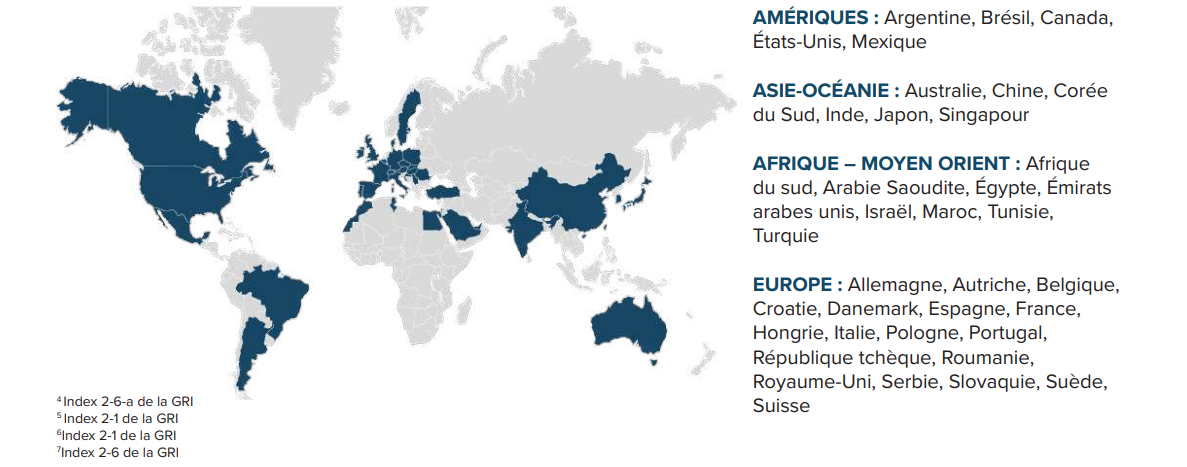
\includegraphics[width=1\linewidth]{Implantation.png}
    \caption{Implantation de SEGULA Technologies à l’échelle internationale}
\end{figure}
\subsection{Fiche signalétique de l'entreprise}
Le tableau ci-dessous présente les données clés du groupe SEGULA Technologies.

\begin{table}[H]
    \centering
    \begin{tabular}{|p{4cm}|p{10cm}|}
        \hline
        \textbf{Raison sociale} & SEGULA Technologies \\ \hline
        \textbf{Forme juridique} & Société par Actions Simplifiée (SAS) \\ \hline
        \textbf{Activité} & Groupe d'ingénierie et de conseil en innovation \\ \hline
        \textbf{Date de création} & 1985, France \\ \hline
        \textbf{Implantations} & 140 implantations dans plus de 30 pays \\ \hline
        \textbf{Adresse du siège} & 19 rue Dares, 92000 Nanterre \\ \hline
        \textbf{Chiffre d'affaires} & Plus de 538 millions d'euros (2023) \\ \hline
        \textbf{Site web} & \url{www.segulatechnologies.com} \\ \hline
    \end{tabular}
    \caption{Fiche signalétique du groupe SEGULA}
\end{table}

\subsection{Mission et chiffre d'affaires}
SEGULA Technologies est le premier groupe européen de conseil et d'ingénierie en innovation technologique. Le groupe intervient sur l'ensemble des phases du cycle de vie d'un projet, depuis sa définition jusqu'à sa concrétisation.
\begin{itemize}
    \item 15 000 collaborateurs et plus de 300 clients industriels majeurs
    \item 2 250 recrutements en 2008, dont 1 500 en France et 750 à l'international
    \item 514 millions d'euros de chiffre d'affaires
    \item 20\% du chiffre d'affaires réalisé à l'international
\end{itemize}
\begin{figure}[H]
    \centering
    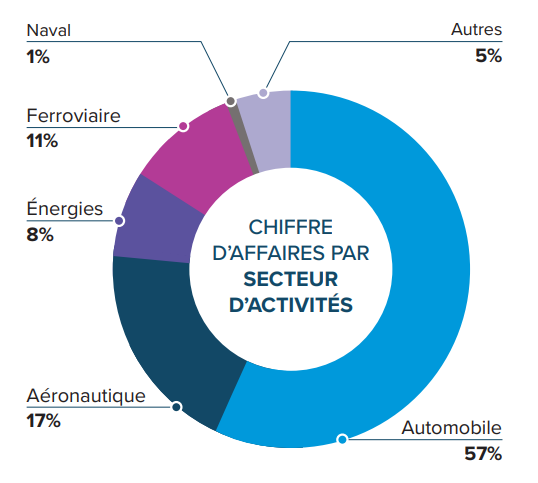
\includegraphics[width=0.5\linewidth]{CA_secteur.png}
    \caption{Répartition du chiffre d’affaires de SEGULA Technologies par secteurs}
\end{figure}

L'activité de SEGULA Technologies s'articule autour de deux axes principaux :
\begin{itemize}
    \item Conseil en technologie et en recherche \& développement
    \item Conseil en organisation et en systèmes d'information
\end{itemize}
\begin{figure}[H]                     
    \centering
    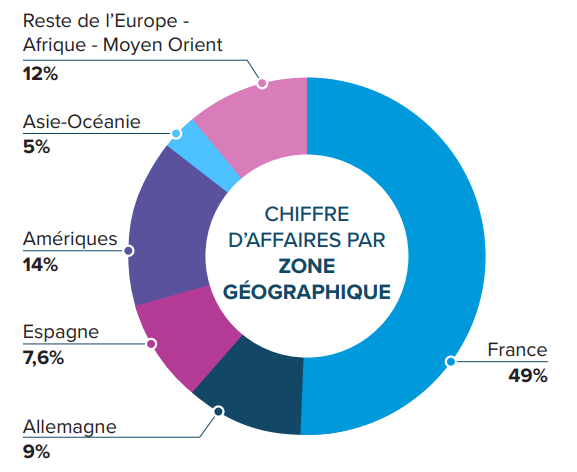
\includegraphics[width=0.5\linewidth]{CA_zone.png}
    \caption{Répartition géographique du chiffre d’affaires de SEGULA Technologies}
\end{figure}

\newpage
\subsection{Secteurs d'activité}
SEGULA Technologies est un groupe d’ingénierie présent à l’échelle internationale, qui ac
compagne la compétitivité des principaux secteurs industriels. Ses interventions couvrent
notamment les domaines de l’automobile, de l’aéronautique, de l’énergie, du rail et du
naval.Lafigure ci-dessous illustre la diversité
des secteurs dans lesquels le groupe opère.
\begin{figure}[H]
    \centering
    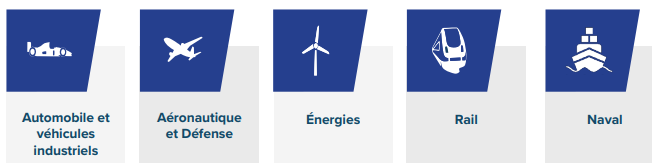
\includegraphics[width=0.5\linewidth]{secteurs.png}
    \caption{Les secteurs d’activitées de SEGULA Groupe}
    \label{fig:placeholder}
\end{figure}
\begin{itemize}
    \item \textbf{Automobile \& Véhicules Industriels} : Présent dans de nombreuses grandes villes à travers le monde, SEGULA Technologies rassemble des milliers de collaborateurs passionnés par le secteur automobile et les véhicules industriels. Les prestations couvrent un large spectre, allant de la gestion de plateformes techniques externalisées à la conception et à l'industrialisation de sous-ensembles.
    \item \textbf{Aéronautique, Aérospatial et Défense} : SIMRA, filiale spécialisée de SEGULA Technologies, a continuellement fait évoluer son offre pour répondre aux exigences croissantes des principaux acteurs des secteurs aéronautique, spatial et de la défense.
    \item \textbf{Énergie} : SEGULA Technologies collabore avec les principaux donneurs d'ordre industriels dans les secteurs de l'énergie nucléaire, thermique et renouvelable.
    \item \textbf{Ferroviaire} : Le groupe apporte son expertise aux industriels du ferroviaire à l'échelle mondiale, intervenant sur l'ensemble du cycle de développement des projets.
    \item \textbf{Naval} : SEGULA Technologies travaille avec les principaux acteurs du secteur naval, couvrant tous types de navires civils, militaires, maritimes et fluviaux.
    \item \textbf{Pétrochimie} : Le groupe soutient les grands donneurs d'ordre du raffinage, de la pétrochimie et de la chimie dès la phase de conception des installations.
    \item \textbf{Pharmacie} : Depuis plus de dix ans, SEGULA Technologies met son expertise au service des principaux acteurs du secteur des sciences de la vie dans leurs projets industriels.
\end{itemize}

\subsection{Clients de SEGULA}
SEGULA Technologies est un acteur majeur de l'ingénierie au service de grands clients industriels. Dans le secteur automobile, Stellantis est reconnu comme l'un de ses principaux partenaires. Le groupe compte également de nombreux autres clients dans les domaines de l'aéronautique, de l'énergie, du ferroviaire et de la pharmacie.

\subsection{SEGULA Technologies Maroc}
\subsubsection{Présentation}
SEGULA Technologies Maroc intervient principalement dans le secteur automobile via ses bureaux d'études situés à Casablanca, Agadir et Tanger, ainsi que dans le secteur aéronautique par l'intermédiaire de sa filiale SIMRA. Dans le domaine automobile, l'entreprise a réalisé de nombreux projets en mode forfaitaire, accompagnant ses clients dans la conception et l'industrialisation de nouveaux produits et la création de nouvelles usines. Dans le secteur aéronautique, SIMRA collabore avec les principaux industriels marocains et internationaux.

\subsubsection{Fiche signalétique de SEGULA Technologies Maroc}
\begin{table}[h!]
    \centering
    \begin{tabular}{|p{4cm}|p{10cm}|}
        \hline
        \textbf{Raison sociale} & SEGULA Technologies Maroc \\ \hline
        \textbf{Forme juridique} & Société Anonyme \\ \hline
        \textbf{Activité} & Groupe d'ingénierie \\ \hline
        \textbf{Date de création} & 2018 \\ \hline
        \textbf{Domaines d'expertise} & Plan de forme Roulage (Kénitra), optimisation des coûts RHN, Conception \\ \hline
        \textbf{Implantations} & - Casablanca Nearshore Park, 1100 Bd. Al Qods, Shore 26, Sidi Maarouf, 20270 Casablanca \newline - Park View Square, La Baie des Palmiers, immeuble 56 Founty, 80010 Agadir \newline - Bureau C1-B, 3e étage, Centre d'Affaires ZF Business Center, lot 40-A, Zone Franche d'Exportation, Tanger \newline - Zone Technopole Aéroport Mohamed V (site de la filiale SIMRA) \\ \hline
        \textbf{Site web} & \url{https://morocco.segulatechnologies.com} \\ \hline
    \end{tabular}
    \caption{Fiche signalétique de SEGULA Technologies Maroc}
\end{table}

\subsubsection{Organigramme de la société}
Une entreprise est une organisation hiérarchique regroupant différentes activités. L'organigramme de SEGULA Technologies Maroc, où s'est déroulé mon stage, est structuré pour permettre une gestion efficace de ses projets.

\subsubsection{Organisation du département « Vehicle Engineering »}
Le département Vehicle Engineering de SEGULA Technologies Maroc joue un rôle central dans le développement de solutions d'ingénierie et de design pour l'industrie automobile. Il regroupe plusieurs équipes spécialisées :

\begin{itemize}
    \item \textbf{Équipe Remontage numérique} : Ce pôle est chargé de la gestion et de la mise à jour des maquettes numériques 3D, base essentielle à la conception et au développement du véhicule. Les ingénieurs assurent la consolidation des données issues des différents sous-systèmes.
    \item \textbf{Équipe Architecture} : Cette équipe est responsable de l'intégration globale des systèmes et sous-systèmes dans le véhicule. Elle prend en compte les contraintes réglementaires, les exigences stylistiques, les contraintes industrielles ainsi que la qualité perçue.
    \item \textbf{Équipe Implantation} : Le pôle Implantation se concentre sur la synthèse géométrique des pièces et sous-systèmes, garantissant leur positionnement optimal dans l'espace véhicule pour éviter les interférences et respecter les règles métier.
\end{itemize}

\section{Contexte général du projet}

\subsection{Problématique}
Dans le secteur du recrutement et des entreprises de services du numérique, la présentation des profils des candidats ou des consultants aux clients finaux revêt une importance capitale. Ce processus implique généralement la conversion des Curriculum Vitae (CV) originaux, souvent hétérogènes en termes de format (documents texte, PDF, images scannées) et de structure, vers un format standardisé propre à l'entreprise, communément appelé "Dossier de Compétences" ou "BioProfile".

Actuellement, cette tâche de transcription et de mise en forme est principalement réalisée de manière manuelle par les équipes des Ressources Humaines (RH) ou les ingénieurs d'affaires. Dans ce cadre dynamique, la gestion et le traitement efficaces de ces documents deviennent cruciaux pour assurer une réactivité commerciale face aux besoins des clients. Mon projet se concentre sur le développement d'un pipeline d'automatisation exploitant l'intelligence artificielle pour traiter ces flux de documents.

Le défi principal réside dans la conception d'un système automatisé qui non seulement ingère et analyse ces données non structurées de manière fiable, mais permet aussi de générer des documents de présentation harmonisés. La problématique se complexifie avec les exigences de précision dans l'extraction des informations clés (compétences, expériences, formations) à partir de formats complexes (tableaux, scans). De plus, l'utilisation de l'intelligence artificielle dans ce domaine nécessite une attention particulière sur la sécurité et la confidentialité des données à caractère personnel, éléments primordiaux dans le secteur du recrutement. La conception du pipeline doit donc être robuste, intelligente et sécurisée pour s'adapter à la diversité des CV reçus.

\subsection{Objectifs de la mission}
Le principal objectif de cette mission est de fournir aux équipes de recrutement et aux ingénieurs d'affaires un outil intelligent leur permettant d'automatiser la création des dossiers de compétences, afin de se concentrer sur des tâches à plus forte valeur ajoutée comme l'évaluation humaine des candidats.

Durant mon projet, j'ai été amenée à :
\begin{enumerate}
    \item Créer un pipeline automatisé d'ingestion et de prétraitement de documents supportant de multiples formats (texte natif et documents scannés).
    \item Implémenter un moteur d'extraction intelligente, basé sur l'intelligence artificielle, capable de comprendre la sémantique d'un CV et d'en extraire les informations pertinentes de manière structurée.
    \item Développer un module de génération automatisée de documents, chargé de formater les données extraites (incluant la photo de profil) dans un modèle de présentation dynamique (PowerPoint).
    \item Concevoir une architecture garantissant le traitement local des données pour assurer une confidentialité et une sécurité totales.
    \item Créer et déployer une interface utilisateur intuitive permettant aux équipes d'interagir facilement avec le système de génération.
\end{enumerate}

\subsection{Enjeux de la mission}
Les enjeux de ce projet sont :
\begin{itemize}
    \item \textbf{Améliorer la productivité :} Favoriser la réactivité commerciale en réduisant drastiquement le temps passé sur des tâches administratives répétitives (la refonte des CV), accélérant ainsi le processus de proposition de profils aux clients.
    \item \textbf{Garantir la sécurité des données :} Assurer la souveraineté et la confidentialité des informations personnelles des candidats en intégrant des modèles d'intelligence artificielle fonctionnant en circuit fermé, répondant ainsi aux normes de sécurité strictes.
    \item \textbf{Standardiser la qualité :} Harmoniser la présentation commerciale des profils de l'entreprise, en éliminant les erreurs humaines liées à la ressaisie et en garantissant un livrable final visuellement irréprochable.
    \item \textbf{Soutenir la transformation digitale :} Contribuer à la modernisation des processus internes des ressources humaines en intégrant des technologies avancées d'analyse de documents et d'intelligence artificielle générative.
\end{itemize}


\section{Planification du projet}

\subsection{Diagramme de GANTT}
Le diagramme de Gantt est l'un des outils les plus efficaces pour faciliter la gestion des projets. Il permet une visualisation claire de l'état d'avancement en spécifiant les dates de début et de fin, ainsi que la durée de chaque tâche. Nous avons utilisé ce diagramme pour la planification complète de notre stage de deux mois (8 semaines). Cette planification resserrée nous a aidé à travailler efficacement et à réaliser le projet dans les délais impartis.

\vspace{1cm}
\begin{figure}[H]
    \centering
    % Ajustement de la taille pour s'adapter à la largeur de la page
    \resizebox{0.95\textwidth}{!}{
    \begin{ganttchart}[
        hgrid,
        vgrid,
        x unit=0.9cm,
        y unit title=0.6cm,
        y unit chart=0.6cm,
        title label font=\bfseries\footnotesize,
        bar label font=\footnotesize,
        group label font=\bfseries\footnotesize,
        bar/.style={fill=blue!50, draw=blue!80, line width=1pt},
        group/.style={fill=gray!80, draw=black},
        progress label text={},
        group right shift=0,
        group top shift=0.6,
        group height=.2,
        group peaks width={0.1}]{1}{8}
        
        \gantttitle{Planification du Projet (8 semaines)}{8} \\
        \gantttitlelist{1,...,8}{1} \\
        
        \ganttgroup{Phase 1 : Analyse \& Besoins}{1}{1} \\
        \ganttbar{Compréhension \& Analyse}{1}{1} \\
        
        \ganttgroup{Phase 2 : Architecture}{2}{2} \\
        \ganttbar{Conception du pipeline}{2}{2} \\
        
        \ganttgroup{Phase 3 : Dév. Extraction \& IA}{3}{5} \\
        \ganttbar{Prétraitement \& OCR}{3}{4} \\
        \ganttbar{Intégration Modèle IA}{4}{5} \\
        
        \ganttgroup{Phase 4 : Génération \& Interface}{6}{7} \\
        \ganttbar{Génération Documentaire}{6}{6} \\
        \ganttbar{Interface Utilisateur}{7}{7} \\
        
        \ganttgroup{Phase 5 : Finalisation}{8}{8} \\
        \ganttbar{Tests, Débogage \& Rapport}{8}{8}
        
    \end{ganttchart}
    }
    \caption{Diagramme de GANTT prévisionnel du projet sur 2 mois}
    \label{fig:gantt_2mois}
\end{figure}
Lors de notre projet, nous avons débuté par une compréhension approfondie de la problématique. Durant la première semaine, nous avons consacré notre temps à analyser les besoins des utilisateurs finaux (équipes RH et commerciaux) et à identifier les défis liés au traitement des CV. Cela impliquait d'examiner les formats de documents reçus et de définir clairement les règles de gestion et les attentes du livrable final.

Ensuite, au cours de la deuxième semaine, nous avons travaillé sur la conception de l'architecture globale du système. Nous avons évalué différentes approches pour l'extraction de texte, la reconnaissance optique de caractères pour les documents scannés, et sélectionné les modèles d'intelligence artificielle les plus adaptés à une exécution locale. Les propositions d'architecture ont été validées pour s'assurer de leur faisabilité sur la durée restante du stage.

Entre la troisième et la cinquième semaine, nous sommes entrés dans la phase principale de réalisation en implémentant le pipeline de prétraitement et d'extraction de données. Cela comprenait le développement des modules permettant de lire les documents, d'isoler les images (comme les photos de profil) et de préparer le texte brut. En parallèle, nous avons configuré et optimisé le moteur d'intelligence artificielle pour qu'il analyse ce texte et restitue les données du candidat sous un format strictement structuré, prêt à être exploité.

Au cours des semaines six et sept, nous nous sommes concentrés sur le module de post-traitement et l'interface utilisateur. Nous avons développé le système chargé de la génération automatisée des présentations, capable d'injecter dynamiquement les données structurées dans le modèle de présentation officiel de l'entreprise. Simultanément, nous avons intégré l'interface web pour rendre ce service accessible et facile d'utilisation pour les équipes métiers.

Enfin, la huitième et dernière semaine a été dédiée à une phase de tests intensifs sur des échantillons réels de CV variés, au débogage final de l'application, et à la rédaction de la documentation et du présent rapport de stage.



\subsection{Méthodologie de réalisation du projet}
La réalisation d'un projet intégrant de l'intelligence artificielle et de l'automatisation de flux documentaires nécessite une méthodologie structurée pour garantir l'atteinte des objectifs métiers. Voici la méthodologie que nous avons adoptée, organisée en plusieurs étapes clés :

\textbf{1. Définition des Objectifs et des Exigences} \\
La première étape consiste à définir clairement les objectifs du projet en termes de résultats et de besoins fonctionnels. Il est essentiel de comprendre quelles informations doivent impérativement figurer sur le document final et comment l'outil s'insérera dans le quotidien des équipes. Cela implique de documenter les exigences de performance, de tolérance aux différents formats de fichiers, et surtout les contraintes strictes de sécurité et de confidentialité des données.

\textbf{2. Analyse et Compréhension des Données} \\
Cette étape implique de recenser et d'analyser la nature des données d'entrée (les CV). Il a fallu examiner la structure, la variabilité des mises en page, l'utilisation de tableaux ou de colonnes, et la présence de documents non textuels (scans). Cette exploration permet d'identifier les limites des méthodes d'extraction classiques et de planifier la mise en place d'outils avancés de vision par ordinateur pour pallier ces problématiques de qualité de données.

\textbf{3. Conception de l'Architecture du Pipeline} \\
À ce stade, il a fallu concevoir un flux de traitement des données adapté aux besoins du projet. Le modèle a été pensé de manière modulaire : un module d'ingestion (lecture multiformat), un module d'intelligence artificielle (analyse sémantique et structuration), et un module de restitution (génération du document final). Chaque choix technologique a été évalué en fonction de sa capacité à fonctionner de manière autonome et sécurisée, sans dépendre de services externes non maîtrisés.

\textbf{4. Développement et Mise en Œuvre} \\
Cette étape correspond à la phase de programmation des processus automatisés. Les développements ont inclus l'écriture des algorithmes de lecture, la mise au point des directives (prompts) envoyées au modèle d'intelligence artificielle pour garantir la précision de l'extraction, ainsi que le développement de la logique d'injection des données dans la présentation cible. Des tests unitaires continus ont été réalisés pour s'assurer que chaque composant du pipeline fonctionnait correctement de manière isolée.

\textbf{5. Déploiement et Interface Utilisateur} \\
Une fois les algorithmes validés, le pipeline a été intégré au sein d'une interface web. Le déploiement s'est fait de manière à rendre l'outil accessible via un simple navigateur, dissimulant la complexité technologique sous-jacente. Il est également essentiel à cette étape de s'assurer de la stabilité du service pour gérer plusieurs requêtes simultanées de la part des utilisateurs.

\textbf{6. Tests, Évaluation et Optimisation} \\
Mettre en place des tests d'intégration complets sur des cas réels (Edge cases) est crucial. En fonction des retours qualitatifs obtenus lors des premiers essais, les algorithmes de détection et les instructions du modèle d'IA ont été ajustés. L'optimisation continue permet d'assurer que le système reste robuste face à l'infinie variété de présentations possibles d'un CV.


\section{Conclusion}
Ce chapitre a posé le cadre général de notre projet de fin d'année, en mettant en lumière les défis liés à la gestion documentaire dans le secteur du recrutement et de l'ingénierie. La refonte manuelle des CV en dossiers de compétences est une tâche chronophage qui freine la réactivité des équipes. Nous avons défini les objectifs de notre mission, visant à créer un écosystème automatisé capable d'analyser intelligemment ces documents et de générer des présentations standardisées, tout en répondant aux enjeux critiques de sécurité des données.

La planification rigoureuse du projet et l'adoption d'une méthodologie modulaire ont permis de structurer notre approche, allant de la compréhension initiale des données non structurées jusqu'au déploiement d'une interface utilisateur intuitive.

À la lumière de cette étude du contexte et des objectifs fixés, il devient évident que pour relever ces défis d'extraction et de génération automatisée, l'intégration de technologies avancées de traitement du langage naturel et d'analyse d'images est cruciale. Le prochain chapitre se penchera sur l'état de l'art des concepts et des technologies de pointe pouvant aider à résoudre ces problématiques, en optimisant la performance de notre pipeline documentaire et en garantissant la qualité des données extraites.

\chapter{Cadre théorique}

Dans ce chapitre, nous approfondissons l'étude de la digitalisation des processus de recrutement, et plus particulièrement l'intégration de l'Intelligence Artificielle dans la gestion des talents. Nous débutons par une définition des concepts de traitement automatique des candidatures et analysons les mécanismes qui régissent la transformation d'un Curriculum Vitae brut en un document commercial exploitable. Nous introduisons ensuite l'application AI-BioProfile, conçue pour enrichir l'écosystème des Ressources Humaines (RH) et des Entreprises de Services du Numérique (ESN) en automatisant les tâches administratives chronophages. Les sections suivantes détaillent la raison d'être de cette solution, articulant sa mission, sa vision, et l'effet escompté sur la productivité des équipes. Le chapitre conclut avec une exploration des différents utilisateurs de l'application, incluant les chargés de recrutement, les ingénieurs d'affaires et les candidats, en examinant leurs interactions au sein de ce processus dynamique.

\section{L'Intelligence Artificielle au service du recrutement}

\subsection{La transformation digitale des Ressources Humaines}
Le secteur du recrutement connaît aujourd'hui une mutation profonde tirée par la transformation digitale. Face à un volume de candidatures toujours plus important et à une concurrence accrue pour attirer les meilleurs talents, les entreprises cherchent à optimiser leurs processus. L'Intelligence Artificielle (IA) s'impose comme une réponse efficace pour traiter de grandes quantités de données non structurées (comme les documents textuels ou les images scannées), permettant ainsi aux professionnels des ressources humaines de se concentrer sur l'humain plutôt que sur la saisie administrative.

\subsection{Le traitement automatique des CV (Resume Parsing)}
Le traitement automatique de CV, ou \textit{Resume Parsing}, est une technologie qui permet de lire, d'analyser et d'extraire intelligemment les informations clés contenues dans un Curriculum Vitae (données de contact, expériences, compétences, diplômes). Cette automatisation s'appuie sur des technologies avancées de traitement du langage naturel (NLP) et de reconnaissance optique de caractères (OCR). Si le candidat rédige son CV dans un format libre (PDF, Word, Image), l'objectif du "parsing" est d'uniformiser ces données pour les rendre exploitables, consultables et formatables selon les standards de l'entreprise recruteuse.


\section{L'application AI-BioProfile}

\subsection{À propos d'AI-BioProfile}
La gestion des dossiers de présentation des consultants est souvent perçue comme une tâche rébarbative et chronophage au sein des cabinets de conseil et des ESN. C'est de ce constat qu'est née l'initiative AI-BioProfile.

Nous avons l'intime conviction que les équipes de recrutement et les ingénieurs d'affaires, lorsqu'ils sont libérés de la charge de la mise en forme documentaire, peuvent allouer un temps précieux à l'accompagnement des candidats et à la satisfaction des exigences clients.

Nous avons mis en commun notre expertise technique pour concevoir un outil ambitieux qui redonne le pouvoir aux recruteurs, en transformant instantanément n'importe quel profil en une présentation percutante.

\textbf{Mission :} Autonomiser les acteurs du recrutement et les commerciaux en leur fournissant une plateforme intelligente capable d'extraire, de structurer et de générer automatiquement des dossiers de compétences (BioProfiles) standardisés à partir de CV hétérogènes.

\textbf{Vision :} Notre vision est de créer un écosystème de recrutement fluide, où les barrières administratives disparaissent grâce à l'automatisation locale et sécurisée. Nous entrevoyons un environnement de travail où les talents sont présentés aux clients finaux de manière rapide, homogène et professionnelle, accélérant ainsi la mise en relation entre les compétences et les opportunités d'affaires.

\subsection{Le concept du "Dossier de Compétences" (BioProfile)}
Dans le domaine des services numériques, le client final ne reçoit que très rarement le CV original du candidat. Il reçoit un "Dossier de Compétences" (ou BioProfile). Il s'agit d'un document anonymisé ou semi-anonymisé, reprenant la charte graphique de l'entreprise qui propose le candidat, et qui met en valeur ses compétences techniques (Hard Skills), comportementales (Soft Skills) et ses expériences de manière uniforme. AI-BioProfile a pour but de générer ce livrable final (au format PowerPoint) de façon entièrement automatisée.


\section{Les utilisateurs de l'application}

Dans le contexte de l'application AI-BioProfile, le diagramme de cas d'utilisation illustré dans la figure 2.1  met en évidence les interactions entre les différents types d'utilisateurs et les fonctionnalités du système.

\textit{(Vous pouvez insérer ici un diagramme de cas d'utilisation UML - Figure 2.1)}

\subsection{Le Chargé de Recrutement (RH)}
Il est l'utilisateur principal du système en back-office. Son rôle est de sourcer les meilleurs profils et de préparer leurs dossiers :
\begin{itemize}
    \item \textbf{Importer des documents :} Il charge les CV originaux des candidats (formats PDF, Word, texte) sur la plateforme.
    \item \textbf{Vérifier et ajuster les données :} Il relit les informations extraites par l'IA (présentées sur l'interface) et peut y apporter des modifications manuelles si nécessaire avant validation.
    \item \textbf{Générer le BioProfile :} Il déclenche la création du document de présentation final.
\end{itemize}

\subsection{L'Ingénieur d'Affaires (Commercial)}
Son rôle est de faire le pont entre les profils recrutés et les besoins des clients de l'entreprise :
\begin{itemize}
    \item \textbf{Exploiter le BioProfile :} Il télécharge les présentations PowerPoint générées par l'outil pour les intégrer dans ses propositions commerciales.
    \item \textbf{Proposer des profils :} Grâce au formatage standardisé, il peut présenter rapidement et professionnellement les candidats aux clients finaux, augmentant ainsi les chances de placement.
\end{itemize}

\subsection{Le Candidat}
Bien qu'il n'interagisse pas directement avec le code de la plateforme, il est à la source de la donnée :
\begin{itemize}
    \item \textbf{Fournir le contenu :} Il soumet son Curriculum Vitae original, quels que soient sa forme et son style de présentation, qui servira de matière première au moteur d'intelligence artificielle.
\end{itemize}

\subsection{Le Client Final}
Il est le destinataire de la valeur générée par le système :
\begin{itemize}
    \item \textbf{Consulter les profils :} Il reçoit et lit le BioProfile finalisé, clair, structuré et visuellement agréable, ce qui facilite sa prise de décision quant à l'acceptation d'un consultant sur son projet.
\end{itemize}


\section{Conclusion}
Ce chapitre a présenté le cadre théorique du stage. L'étude sur la transformation digitale des ressources humaines a mis en lumière l'importance de l'automatisation dans le traitement des candidatures. L'application AI-BioProfile se distingue par son approche intégrée, offrant à la fois un gain de temps considérable et une standardisation documentaire irréprochable. Nous avons exploré la mission de l'outil, sa vision future, et l'impact attendu sur le processus de placement des consultants. L'analyse des différents utilisateurs du système a montré que chaque acteur, du candidat au client final, bénéficie directement ou indirectement de cette chaîne de valeur optimisée, soulignant le rôle essentiel d'AI-BioProfile dans l'écosystème de l'entreprise.

\chapter{État de l'art}

Dans ce chapitre, nous explorons les diverses technologies et méthodologies qui forment le socle des systèmes d'information modernes orientés vers l'intelligence artificielle et l'automatisation documentaire. L'accent est mis sur des concepts fondamentaux tels que le Traitement du Langage Naturel (NLP), les Grands Modèles de Langage (LLM), la Vision par Ordinateur (Computer Vision), la Reconnaissance Optique de Caractères (OCR), ainsi que sur les architectures d'API modernes. Ces technologies jouent un rôle crucial dans la capacité des entreprises à traiter massivement des données non structurées (comme les CV) pour les transformer en informations structurées et exploitables. Chaque section détaille une technologie spécifique, expliquant son fonctionnement, ses applications et son importance dans le développement d'outils d'automatisation. Ce cadre théorique est essentiel pour comprendre les briques technologiques qui ont permis la conception de l'application AI-BioProfile.

\section{Intelligence Artificielle et Modèles de Langage (LLMs)}

\subsection{Le Traitement du Langage Naturel (NLP)}
Le Traitement du Langage Naturel (en anglais NLP pour \textit{Natural Language Processing}) est une branche de l'intelligence artificielle qui vise à donner aux ordinateurs la capacité de comprendre, d'interpréter et de générer le langage humain de manière significative et utile. Dans le domaine des ressources humaines, le NLP est la technologie fondamentale derrière le "Resume Parsing" (analyse de CV).

Historiquement basé sur des règles statistiques complexes et des expressions régulières (Regex), le NLP moderne s'appuie désormais sur des réseaux de neurones profonds. Il permet d'identifier l'intention d'un texte, d'en extraire les entités nommées (NER - \textit{Named Entity Recognition} : identifier une entreprise, un poste, une école) et d'établir des relations sémantiques entre les mots, peu importe la façon dont le candidat a rédigé son document.

\subsection{Les Grands Modèles de Langage (LLMs)}
Un Grand Modèle de Langage (LLM - \textit{Large Language Model}) est un système d'intelligence artificielle entraîné sur des quantités massives de textes (souvent l'intégralité du web public). Grâce à l'architecture \textit{Transformer}, introduite en 2017, ces modèles ont acquis une capacité exceptionnelle à comprendre le contexte et à générer du texte cohérent (ex: GPT, BERT, Llama, Mistral).

Dans le cadre d'un système d'extraction de données, un LLM ne se contente pas de chercher des mots-clés ; il comprend la structure d'une phrase. Par exemple, il sait différencier "J'ai développé un outil en Python" (compétence acquise) de "J'aimerais apprendre Python" (souhait futur).

\textbf{Inférence Cloud vs Inférence Locale (On-Premise)}
Actuellement, l'utilisation des LLMs se divise en deux grandes approches :
\begin{itemize}
    \item \textbf{Les solutions Cloud (ex: API OpenAI) :} Elles offrent des modèles extrêmement puissants mais nécessitent d'envoyer les données sur des serveurs distants, ce qui pose de graves problèmes de confidentialité (RGPD), particulièrement pour des données sensibles comme des CV.
    \item \textbf{L'inférence locale (ex: Ollama, Mistral) :} Elle permet d'exécuter des modèles de langage puissants et open-source directement sur les serveurs ou les machines de l'entreprise. Cette méthode garantit une souveraineté totale des données, l'information ne quittant jamais le réseau local. C'est un prérequis de plus en plus exigé par les entreprises travaillant avec des données personnelles.
\end{itemize}

\subsection{Le Prompt Engineering et la structuration des données}
Le \textit{Prompt Engineering} (ou ingénierie de requête) est la discipline qui consiste à concevoir et optimiser les instructions envoyées à un LLM pour obtenir le résultat le plus précis possible. Dans les applications métier, on demande souvent au LLM de ne pas répondre par une simple phrase, mais de générer une structure de données stricte (comme le format JSON) pour qu'elle soit exploitable par le reste du code. 

L'utilisation d'outils de validation de schémas (tels que \textit{Pydantic} en Python) permet de forcer le modèle d'IA à respecter des types de données stricts (exiger qu'une date soit au format JJ/MM/AAAA ou qu'une liste de compétences soit sous forme de tableau), garantissant ainsi la stabilité de l'application logicielle qui dépend de cette IA.


\section{Vision par Ordinateur et Traitement Documentaire}

Outre le texte, les documents professionnels comme les CV contiennent souvent des éléments graphiques. La Vision par Ordinateur (\textit{Computer Vision}) est le domaine de l'IA qui permet aux machines "d'ordonner" et de comprendre des images.

\subsection{La Reconnaissance Optique de Caractères (OCR)}
La Reconnaissance Optique de Caractères (OCR) est une technologie permettant de convertir différents types de documents (scans, fichiers PDF non natifs, images capturées par un appareil photo) en données textuelles modifiables et interrogeables. 

Lorsqu'un candidat soumet un CV qui a été scanné ou qui est une simple image, les parseurs de texte classiques sont incapables de lire son contenu. L'OCR (comme le moteur \textit{Tesseract}, soutenu par Google) intervient en analysant les pixels de l'image pour y détecter des formes correspondant à des lettres, puis reconstitue les mots et les phrases. L'intégration de l'OCR est une étape de prétraitement vitale pour assurer que le système ne rejette aucun document sous prétexte de son format.

\subsection{La détection faciale (Facial Detection)}
La détection faciale est une technologie de vision par ordinateur qui permet d'identifier la présence et l'emplacement de visages humains dans des images numériques. Contrairement à la reconnaissance faciale (qui identifie "qui" est la personne), la détection faciale se contente de trouver un visage.

Dans le contexte du traitement de CV, cette technologie (souvent implémentée via des bibliothèques comme \textit{OpenCV} utilisant les classificateurs en cascade de Haar ou des réseaux de neurones) permet de parcourir un document PDF, de repérer automatiquement la photo de profil du candidat, de la recadrer et de l'isoler afin de l'insérer plus tard dans le dossier de compétences généré.

\subsection{Le parsing de documents complexes (PDF, DOCX)}
L'extraction de données passe par des bibliothèques logicielles capables de disséquer des formats propriétaires complexes :
\begin{itemize}
    \item \textbf{Le format PDF :} Considéré comme le standard d'affichage, c'est l'un des formats les plus difficiles à analyser car il ne structure pas sémantiquement l'information (il positionne des caractères sur des coordonnées X et Y). L'utilisation d'outils d'extraction (comme \textit{PyMuPDF}) permet de reconstruire les blocs de texte et de récupérer les objets graphiques intégrés au document.
    \item \textbf{Le format DOCX (Word) :} Basé sur des archives XML, il demande un traitement différent pour parser les paragraphes, les tableaux et extraire les médias (fichiers images stockés dans l'archive).
\end{itemize}


\section{Architecture Web et Génération Documentaire}

\subsection{Les API RESTful et le framework FastAPI}
Une API (Interface de Programmation d'Application) RESTful est une architecture standardisée permettant à différents systèmes informatiques de communiquer entre eux via le protocole HTTP. Dans le cadre des systèmes d'intelligence artificielle, l'API sert de pont entre l'interface utilisateur (Front-end) et les lourds traitements algorithmiques (Back-end).

\textit{FastAPI} est un framework web moderne et très performant développé en Python. Il est particulièrement plébiscité dans les projets liés à la Data Science et à l'IA pour plusieurs raisons :
\begin{itemize}
    \item \textbf{Asynchronisme :} Il gère de manière native la programmation asynchrone, ce qui est indispensable lors des appels à des modèles d'IA qui peuvent prendre plusieurs secondes à répondre, évitant ainsi le blocage du serveur.
    \item \textbf{Validation automatique :} En lien avec la structuration des données (Pydantic), il valide automatiquement les requêtes entrantes et sortantes, réduisant considérablement les erreurs de traitement.
    \item \textbf{Performance :} Conçu pour être l'un des frameworks Python les plus rapides, il rivalise avec des technologies basées sur NodeJS ou Go.
\end{itemize}

\subsection{La génération automatisée de présentations}
Une fois la donnée extraite et validée par l'IA, le système d'information doit restituer une valeur ajoutée exploitable pour l'utilisateur. La génération dynamique de documents repose sur l'interaction logicielle avec les standards de l'industrie (comme le standard \textit{Office Open XML} de Microsoft).

Grâce à des bibliothèques de manipulation (telles que \textit{python-pptx}), il est possible d'éditer programmatiquement des présentations PowerPoint. Le système peut ouvrir un modèle de présentation d'entreprise (Template), repérer des marqueurs spécifiques, et injecter dynamiquement le texte structuré (expériences, compétences) ainsi que les images (photo de profil extraite) en respectant parfaitement la typographie et la charte graphique définies. Cela constitue l'étape finale du pipeline d'automatisation.


\section{Conclusion}

Dans ce chapitre, nous avons défini les concepts fondamentaux et les briques technologiques qui rendent possible l'automatisation intelligente des flux documentaires. Nous avons exploré comment le Traitement du Langage Naturel (NLP) et les Grands Modèles de Langage locaux permettent une compréhension profonde et sécurisée des données textuelles. De plus, nous avons mis en évidence l'importance critique de la Vision par Ordinateur (OCR et détection faciale) pour pallier la diversité des formats de CV, ainsi que le rôle essentiel des API modernes (FastAPI) et de la génération documentaire programmatique pour fournir un service complet de bout en bout. 

Cette exploration théorique démontre la maturité de ces technologies pour résoudre des problématiques d'affaires concrètes. Le prochain chapitre procédera à une analyse approfondie des besoins de notre projet et détaillera l'étude technique de mise en œuvre, expliquant comment ces technologies ont été spécifiquement architecturées et orchestrées pour donner naissance à l'application AI-BioProfile.
```

\chapter{Analyse des besoins et étude technique}

Dans ce chapitre, nous allons étudier l'environnement du recrutement et de la gestion documentaire au sein de l'entreprise afin de comprendre les différentes contraintes liées au traitement des CV. Ensuite, nous procéderons à l'analyse approfondie des besoins, en vue de les synthétiser et de proposer une architecture logicielle adaptée et efficace. Nous réaliserons par la suite une étude technique qui fournira une vue d'ensemble des technologies, des processus, et des outils évalués pour concevoir, développer et mettre en œuvre le projet AI-BioProfile. L'objectif principal de cette étude est de déterminer la faisabilité technique du projet, de justifier nos choix architecturaux et d'identifier les solutions les plus appropriées pour répondre aux exigences strictes de performance et de sécurité des données.

\section{Compréhension et recueil des informations sur les besoins}

\subsection{Compréhension de la nature des besoins}
Dans le cadre de mon projet de fin d'année, j'ai eu la responsabilité de conceptualiser et de réaliser une application complète d'intelligence artificielle pour automatiser la génération des dossiers de compétences (BioProfiles). Le processus de recrutement actuel implique la réception quotidienne de dizaines de CV sous des formats hétérogènes. La conversion manuelle de ces documents en présentations commerciales standardisées est une tâche à faible valeur ajoutée, source d'erreurs et de retards dans la proposition des candidats aux clients.

La solution à concevoir doit couvrir différents aspects du traitement de la donnée non structurée, en tenant compte des contraintes opérationnelles :
\begin{itemize}
    \item L'application doit être capable de lire et d'interpréter des formats de fichiers variés (PDF texte, PDF scannés, documents Word DOCX).
    \item L'extraction des données doit être sémantique (comprendre les expériences et compétences) et non basée sur de simples mots-clés.
    \item Le système doit garantir la confidentialité absolue des données des candidats, excluant de facto l'utilisation d'API d'intelligence artificielle hébergées sur le Cloud public.
    \item La restitution doit être immédiate et directement exploitable sous la forme d'un fichier PowerPoint respectant la charte graphique de l'entreprise.
\end{itemize}

\subsection{Recueil des informations sur les besoins}
Les réunions avec les différentes parties prenantes (Ressources Humaines, Ingénieurs d'Affaires) ont permis d'identifier et de segmenter les besoins en plusieurs modules architecturaux distincts :

\textbf{Module 1 : Pipeline d'ingestion et de prétraitement documentaire}
L'objectif est de préparer la donnée brute pour qu'elle soit lisible par l'intelligence artificielle. Cela nécessite de :
\begin{itemize}
    \item Concevoir un système d'extraction de texte natif et d'analyse d'images (Computer Vision) pour récupérer la photo de profil.
    \item Intégrer un système de Reconnaissance Optique de Caractères (OCR) robuste pour traiter les CV scannés.
\end{itemize}

\textbf{Module 2 : Pipeline d'inférence et d'Intelligence Artificielle}
L'objectif est d'analyser le texte extrait pour en dégager une structure de données claire. Cela implique de :
\begin{itemize}
    \item Déployer un modèle de langage (LLM) en local sur les serveurs de l'entreprise.
    \item Concevoir des instructions (Prompts) strictes pour forcer le modèle à renvoyer un format JSON précis (Nom, Titre, Compétences, Expériences).
\end{itemize}

\textbf{Module 3 : Pipeline de post-traitement et génération}
L'objectif est de convertir la donnée structurée en un livrable commercial. Cela nécessite de :
\begin{itemize}
    \item Développer un script capable de manipuler le format Office Open XML pour injecter du texte et des images dans un modèle PowerPoint existant.
\end{itemize}

\textbf{Module 4 : Interface Utilisateur et API}
L'objectif est de rendre le service accessible aux utilisateurs non techniques. Cela implique de :
\begin{itemize}
    \item Développer une API asynchrone capable de gérer plusieurs requêtes simultanées.
    \item Créer une interface web (Front-end) intuitive permettant le chargement (upload) des CV et la prévisualisation des données avant la génération finale.
\end{itemize}


\section{Identification des besoins}

Suite au recueil des informations, les exigences du projet ont été classifiées en deux catégories : les besoins fonctionnels (ce que le système doit faire) et les besoins non fonctionnels (comment le système doit se comporter).

\subsection{Besoins fonctionnels}
\begin{itemize}
    \item \textbf{Gestion de l'import de fichiers :} Le système doit permettre le téléchargement de fichiers aux formats PDF, DOCX et TXT.
    \item \textbf{Extraction multimodale :} Le système doit extraire non seulement le texte, mais aussi isoler et recadrer automatiquement la photo de profil du candidat présente sur le document.
    \item \textbf{Validation humaine dans la boucle (Human-in-the-loop) :} Avant de générer le fichier PowerPoint final, l'utilisateur doit pouvoir visualiser les données extraites par l'IA sur l'interface web, et corriger manuellement d'éventuelles erreurs ou omissions.
    \item \textbf{Génération du livrable :} Le système doit permettre le téléchargement direct du BioProfile au format .pptx, correctement formaté.
\end{itemize}

\subsection{Besoins non fonctionnels}
\begin{itemize}
    \item \textbf{Sécurité et Confidentialité (Privacy-by-design) :} C'est le besoin le plus critique. Les CV contiennent des données sensibles (RGPD). Aucune donnée textuelle ou image ne doit transiter par des serveurs externes. Les algorithmes d'IA doivent tourner en local (On-Premise).
    \item \textbf{Temps de réponse (Performance) :} L'ensemble du processus (du chargement du CV à la génération du PowerPoint) doit s'effectuer dans un délai raisonnable (idéalement inférieur à une minute) pour maintenir une expérience utilisateur fluide, malgré la lourdeur des traitements d'IA locale.
    \item \textbf{Résilience et fiabilité :} Le système doit être capable de détecter si un PDF est illisible (ex: scan de très mauvaise qualité) et renvoyer des messages d'erreur clairs à l'utilisateur sans faire crasher l'application.
\end{itemize}


\section{Étude Technique}

Afin de construire une architecture robuste répondant à ces besoins complexes, nous avons réalisé un benchmark des technologies disponibles sur le marché pour chaque brique de notre application. Les critères d'évaluation incluent la performance, la facilité d'intégration, le coût (licence), et surtout la capacité à fonctionner hors-ligne (localement).

\subsection{Benchmark et analyse des outils}

\textbf{1. Comparaison des outils d'extraction PDF}
Pour extraire le texte et les images des fichiers PDF, nous avons évalué :
\begin{itemize}
    \item \textit{PyMuPDF (fitz) :} Extrêmement rapide, écrit en C, il gère parfaitement les coordonnées spatiales du texte et l'extraction native des images.
    \item \textit{PyPDF2 :} Populaire et 100\% Python, mais nettement plus lent et souvent mis en échec par des formats de PDF récents.
    \item \textit{PDFMiner :} Très précis sur l'extraction de texte complexe, mais extrêmement lourd et lent, inadapté à un traitement quasi-temps réel.
\end{itemize}
\textit{Choix : PyMuPDF a été sélectionné pour ses performances supérieures et sa flexibilité dans l'extraction des images.}

\textbf{2. Comparaison des moteurs d'OCR (Reconnaissance Optique)}
\begin{itemize}
    \item \textit{Tesseract OCR :} Solution open-source soutenue par Google, très mature, supportant de nombreuses langues, fonctionnant parfaitement en local.
    \item \textit{EasyOCR :} Basé sur le Deep Learning (PyTorch), il est très précis mais nécessite une grande puissance de calcul (GPU) pour être rapide, ce qui l'alourdit.
    \item \textit{Google Cloud Vision API :} La meilleure précision du marché, mais éliminée d'office en raison de la contrainte de confidentialité des données (solution Cloud).
\end{itemize}
\textit{Choix : Tesseract OCR a été retenu pour son excellent compromis entre vitesse d'exécution sur CPU, gratuité et respect de la confidentialité.}

\textbf{3. Comparaison des moteurs d'Inférence IA (LLM Local)}
\begin{itemize}
    \item \textit{Ollama (avec modèle Mistral) :} Un outil open-source permettant d'exécuter facilement des grands modèles de langage en local. Le modèle Mistral offre des performances comparables à GPT-3.5 tout en étant assez léger pour tourner sur des machines standards.
    \item \textit{OpenAI API (ChatGPT) :} Très facile à implémenter et ultra-performant pour structurer du JSON, mais enfreint la règle de souveraineté des données exigée par le projet.
    \item \textit{Llama.cpp :} Très optimisé, mais plus complexe à mettre en place en tant qu'API de service (backend) par rapport à la simplicité d'Ollama.
\end{itemize}
\textit{Choix : Ollama couplé au modèle Mistral a été choisi car il permet une inférence 100\% locale, garantissant la sécurité des données tout en offrant une précision sémantique élevée.}

\textbf{4. Comparaison des Frameworks Backend Web (Python)}
\begin{itemize}
    \item \textit{FastAPI :} Framework moderne, nativement asynchrone, ultra-rapide. Il s'intègre parfaitement avec \textit{Pydantic} pour la validation stricte des données (JSON), ce qui est idéal pour communiquer avec un LLM.
    \item \textit{Flask :} Très simple et léger, mais la gestion asynchrone (nécessaire pour ne pas bloquer le serveur pendant que l'IA réfléchit) est moins native et moins performante que FastAPI.
    \item \textit{Django :} Framework extrêmement complet (Batteries-included), mais beaucoup trop lourd pour notre besoin qui se concentre sur la création d'une API de traitement de données.
\end{itemize}
\textit{Choix : FastAPI s'est imposé comme une évidence pour ses performances asynchrones et sa synergie avec Pydantic.}


\subsection{Définitions des Outils Choisis dans l'Architecture}

\textbf{FastAPI et Pydantic} \\
FastAPI est un framework web moderne et rapide pour la création d'API avec Python, basé sur les annotations de type standard de Python. Dans notre architecture, il agit comme le chef d'orchestre. Il réceptionne les requêtes des utilisateurs contenant les CV, distribue les tâches d'extraction aux différents modules, et renvoie le fichier PowerPoint final. Couplé à la bibliothèque \textit{Pydantic}, il nous permet de définir des schémas de données stricts (par exemple, obliger le LLM à retourner une liste d'expériences contenant spécifiquement une date, un titre et une description). Si le modèle d'IA tente de renvoyer une donnée mal formatée, Pydantic la rejette et force la validation.

\textbf{Ollama et le modèle Mistral} \\
Ollama est un outil open-source qui simplifie considérablement l'exécution locale de grands modèles de langage (LLMs). Il gère l'allocation mémoire et fournit une API REST locale. Dans notre pipeline, Ollama exécute le modèle franco-européen \textit{Mistral}. Ce modèle est sollicité pour lire le texte brut et désordonné du CV, en comprendre la sémantique, et structurer les données. Cette approche garantit que la "réflexion" de l'intelligence artificielle se fait à huis clos, sur la machine hôte, assurant une conformité totale en matière de protection des données (RGPD).

\textbf{PyMuPDF, Tesseract et OpenCV (Extraction et Vision)} \\
Ce triptyque forme notre moteur d'ingestion documentaire :
\begin{itemize}
    \item \textbf{PyMuPDF} parcourt le fichier PDF pour en extraire le texte natif très rapidement.
    \item Si le texte natif est insuffisant (cas d'un CV scanné), \textbf{Tesseract OCR} prend le relais pour "lire" les pixels de l'image et reconstituer le texte de secours.
    \item \textbf{OpenCV} (via les classificateurs de Haar) intervient en dernier recours pour analyser la géométrie de la page et détecter la présence d'un visage humain. Une fois détecté, le visage est recadré et sauvegardé temporairement pour devenir la photo de profil du document final.
\end{itemize}

\textbf{Python-pptx} \\
C'est une bibliothèque Python dédiée à la création et à la mise à jour de fichiers PowerPoint (.pptx). Dans notre architecture, elle représente la dernière étape du traitement. Le script charge un \textit{Template} (modèle vierge de l'entreprise), accède aux différentes diapositives (Slides) de manière programmatique (via l'XML sous-jacent), et remplace les balises fictives par les véritables données JSON validées (nom, compétences) ainsi que par la photo isolée précédemment.


\section{Conclusion}

L'analyse des besoins et l'étude technique réalisées dans ce chapitre ont permis de cerner avec précision les exigences complexes liées à l'automatisation de la gestion des CV. Nous avons identifié des contraintes fortes, particulièrement en matière de sécurité et de confidentialité, excluant le recours à la facilité des services Cloud. Grâce à un benchmark rigoureux, nous avons sélectionné une stack technologique performante et innovante : FastAPI pour l'orchestration asynchrone, PyMuPDF et Tesseract pour l'ingestion multimodale, Ollama/Mistral pour l'analyse intelligente locale, et python-pptx pour la génération du livrable. 

La faisabilité technique du projet AI-BioProfile est ainsi confirmée. Cette combinaison d'outils open-source garantit non seulement la protection des données, mais offre également les performances nécessaires pour transformer de manière transparente un document brut en un profil commercial qualitatif. En se basant sur ces fondations technologiques solides, le prochain chapitre se concentrera sur la phase de réalisation concrète, en détaillant l'architecture implémentée, les étapes de développement, et les résultats obtenus lors des phases de test.
```
\chapter{Réalisation et Implémentation technique}

Dans ce chapitre, nous détaillons de manière exhaustive et rigoureuse les défis techniques rencontrés ainsi que les solutions algorithmiques implémentées pour aboutir au pipeline final de l'application \textbf{AI-BioProfile}. Le développement de cette solution n'a pas consisté en un simple assemblage de bibliothèques, mais a nécessité l'ingénierie d'une architecture logicielle complexe. Nous avons dû intégrer et optimiser plusieurs disciplines avancées de l'informatique moderne : l'analyse documentaire bas niveau, la vision par ordinateur, l'inférence locale d'intelligence artificielle générative multimodale (VLM), le développement backend asynchrone pour la scalabilité, et enfin la rétro-ingénierie d'arbres XML complexes.

Cette phase de réalisation a été menée en suivant une méthodologie itérative (proche d'Agile), nous permettant de concevoir des prototypes (Proof of Concept), d'identifier rapidement les impasses technologiques (comme les limites de l'extraction de texte classique), et d'opérer des pivots architecturaux décisifs.

\section{Module 1 : Le Moteur d'Ingestion et de Traitement Documentaire}

La première brique fondamentale de notre pipeline consiste à ingérer un document brut (le Curriculum Vitae du candidat) et à le préparer mathématiquement pour l'analyse sémantique. Les CV reçus par les recruteurs de SEGULA Technologies proviennent de sources extrêmement diverses et ne respectent absolument aucun standard de mise en page. 

\subsection{Problématique des formats et choix de l'analyseur PDF}
Un fichier PDF n'est pas conçu pour stocker du texte structuré, mais pour garantir une restitution visuelle fidèle à l'impression, quelles que soient la machine et la police installée. Techniquement, un PDF place des caractères isolés ou des blocs de glyphes à des coordonnées précises (X, Y) sur une page blanche. 
Pour extraire ces informations, nous avons sélectionné la bibliothèque \texttt{PyMuPDF} (aussi connue sous le nom de \texttt{fitz}). Écrite en C++, elle offre une vitesse d'exécution inégalée et permet non seulement d'extraire le texte, mais surtout d'interagir avec les structures de données sous-jacentes du PDF : les images embarquées (XObjects) et les polices vectorielles.

Lorsque l'utilisateur soumet un document (via une requête multipart/form-data), le système l'enregistre temporairement. S'il s'agit d'un fichier Microsoft Word (\texttt{.docx}), nous utilisons une bibliothèque dédiée pour extraire les paragraphes XML. S'il s'agit d'un PDF, le document est chargé en mémoire vive.

\subsection{Extraction de la photo de profil : Une double heuristique}
L'un des défis majeurs a été l'extraction automatisée et isolée de la photo de profil du candidat, un élément indispensable pour la génération de la présentation commerciale (BioProfile) finale. Les CV modernes sont extrêmement graphiques : ils contiennent de multiples éléments visuels tels que des logos d'entreprises, des icônes de réseaux sociaux (LinkedIn, GitHub), des images de fond ou des séparateurs graphiques.

Pour résoudre ce problème de manière totalement robuste et déterministe, nous avons développé un algorithme de filtrage hybride, implémenté sous forme d'un pipeline de scoring :

\subsubsection{Phase 1 : L'approche Heuristique par Scoring Matriciel}
Dans un premier temps, l'algorithme parcourt les métadonnées du PDF pour extraire toutes les images (objets pixellisés) encapsulées. Pour chaque image $i$ extraite, le système calcule un score de confiance $S(i)$ basé sur trois composantes mathématiques :

\begin{itemize}
    \item \textbf{Le ratio d'aspect (Forme) :} Les photos d'identité ou de profil respectent des normes universelles : elles sont généralement carrées ou légèrement rectangulaires (format portrait). Soit $W$ la largeur et $H$ la hauteur de l'image en pixels. Nous calculons le ratio $R = W / H$. Si $R$ est compris entre 0.7 et 1.2, l'image reçoit un bonus. Si $R > 2.0$ (ce qui correspond souvent à un bandeau ou une ligne de séparation), l'image est pénalisée ou exclue.
    \item \textbf{La taille surfacique (Résolution) :} Les icônes ont une surface très faible (souvent inférieure à 50x50 pixels), tandis que les images de fond couvrent des millions de pixels. Soit $A = W \times H$ l'aire de l'image. Nous appliquons une fonction de filtre passe-bande retenant les images dont l'aire correspond à la taille standard d'une photo (entre 10 000 et 400 000 pixels carrés).
    \item \textbf{La position spatiale :} Sur un CV conventionnel, la photo est presque systématiquement positionnée dans le tiers supérieur de la première page. \texttt{PyMuPDF} nous fournit les coordonnées (Bounding Box) de l'image. Si la coordonnée Y se trouve dans la zone supérieure (Top 30\%), le score est augmenté.
\end{itemize}

L'image qui obtient le score final le plus élevé est retenue, sous condition que ce score dépasse un seuil paramétré empiriquement.

\subsubsection{Phase 2 : Le Fallback par Computer Vision (OpenCV)}
Bien que très performante, l'approche heuristique échoue inévitablement dans un cas précis : lorsque le document soumis est un scan complet. Dans cette situation, le fichier PDF ne contient pas de multiples images, mais une seule grande image (la page entière numérisée). Les métadonnées ne nous sont d'aucune utilité.

Pour pallier cette limitation critique, nous avons intégré un système de secours (Fallback) utilisant l'intelligence artificielle spécialisée dans la vision par ordinateur, grâce à la bibliothèque \textbf{OpenCV}. L'algorithme se déroule comme suit :
\begin{enumerate}
    \item L'image complète du scan est chargée sous forme de matrice NumPy et convertie en niveaux de gris pour accélérer le traitement.
    \item Nous appliquons un algorithme basé sur la méthode de Viola-Jones, en utilisant un classificateur \texttt{Haar Cascade} pré-entraîné (\texttt{haarcascade\_frontalface\_default.xml}).
    \item Les hyperparamètres sont strictement définis (par exemple, \texttt{scaleFactor=1.1} et \texttt{minNeighbors=5}) pour limiter les faux positifs.
    \item Lorsque l'algorithme détecte un visage, il renvoie les coordonnées du carré strict l'entourant. Étant donné qu'une photo de profil professionnelle inclut généralement les épaules et le cou, notre algorithme applique un calcul de marge ("Padding") de +30\% sur les bords extérieurs, afin de recadrer l'image intelligemment avant de l'enregistrer.
\end{enumerate}

\begin{figure}[H]
    \centering
    \vspace{8cm} % Espace pour insérer le screenshot
    \caption{Extraction de photo : (Gauche) Échec de l'heuristique sur un scan, (Droite) Recadrage réussi par détection faciale OpenCV.}
    \label{fig:photo_extraction}
\end{figure}


\section{Module 2 : Le Moteur Sémantique et la Transition vers le Multimodal}

Le cœur de la valeur ajoutée de l'application réside dans sa capacité à comprendre le contenu textuel et sémantique du CV. C'est ici que l'intelligence artificielle générative entre en jeu. Durant la phase de conception, cette brique architecturale a fait l'objet d'un pivot majeur.

\subsection{La première itération : L'approche LLM Textuelle Classique}
Initialement, nous avons conçu un pipeline d'extraction séquentiel. Le texte du CV était extrait de manière linéaire (de haut en bas, de gauche à droite) via PyMuPDF. Si le document était un scan, nous utilisions Tesseract OCR pour reconstruire le texte. Le résultat consistait en une très longue chaîne de caractères non formatée, souvent truffée de sauts de lignes illogiques.

Cette chaîne était ensuite injectée dans le contexte ("Prompt") d'un Grand Modèle de Langage (LLM), exécuté localement (pour des raisons de confidentialité) avec le moteur \texttt{Ollama} et le modèle \textit{Mistral}. 
L'instruction donnée à l'IA était : "Analyse le texte de ce CV et retourne les expériences et compétences au format JSON".

\subsubsection{Les limites de l'extraction linéaire}
Après avoir testé ce premier prototype sur un échantillon de 50 CV réels de consultants SEGULA, les résultats se sont avérés insuffisants, en particulier sur les CV d'ingénieurs (très denses et souvent mis en page avec Canva). Nous avons identifié deux écueils bloquants :

\begin{itemize}
    \item \textbf{La perte d'intégrité spatiale (Problème du Multi-colonnes) :} Lorsqu'un algorithme classique lit un PDF divisé en deux colonnes, il lit géométriquement la ligne horizontale. Par exemple, si la colonne de gauche indique la date "2021-2023" et que la colonne de droite indique "Compétence : Python", le texte extrait sera "2021-2023 Compétence : Python". Le LLM, recevant ce texte fusionné, était incapable de reconstituer la logique temporelle des expériences du candidat, associant des entreprises aux mauvaises dates.
    \item \textbf{La destruction de l'information graphique (Problème des Jauges) :} De plus en plus de candidats évaluent leurs compétences à travers des jauges visuelles (par exemple, 4 barres pleines sur 5 pour indiquer un niveau de maîtrise avancé en Java). L'extracteur de texte ne voyant que des pixels vectoriels, il ignorait ces jauges. Le LLM recevait le mot "Java" sans aucune indication de niveau, provoquant une immense perte d'information.
\end{itemize}

\begin{figure}[H]
    \centering
    \vspace{7cm} % Espace pour insérer le screenshot
    \caption{Console de débogage montrant la destruction de la logique d'un texte multi-colonnes lors du parsing linéaire.}
    \label{fig:llm_failure}
\end{figure}


\subsection{La seconde itération : L'approche Vision-Language Model (VLM)}
Face à cette impasse, il est apparu évident que la perte d'informations se situait à la racine de la chaîne : la traduction d'un document 2D en texte 1D. Nous avons donc décidé de faire évoluer l'architecture en intégrant un VLM (Modèle Multimodal), capable d'interpréter simultanément le langage et l'image.

\subsubsection{L'implémentation de l'encodeur Base64}
Au lieu d'extraire uniquement le texte, notre nouveau script (\texttt{extraction\_lmstudio.py}) génère un rendu photographique (Rasterization) de chaque page du PDF. Afin d'éviter de saturer la mémoire du serveur d'inférence (VRAM), les images sont redimensionnées tout en conservant une résolution suffisante pour la lecture du texte, puis encodées en chaînes de caractères \texttt{Base64}.

Lors de l'appel à l'API du modèle (utilisant une compatibilité avec l'API OpenAI), nous transmettons un objet complexe (Array) comprenant à la fois le texte brut (en tant que "Filet de sécurité" ou "Hint") et les images encodées représentant le document dans son aspect d'origine.

\subsubsection{Les bénéfices immédiats du VLM}
Le modèle VLM analyse la requête de manière spatiale. Il "regarde" le document comme le ferait un recruteur humain. Il repère visuellement la séparation des colonnes, il associe graphiquement une date à un bloc de texte en étudiant les marges, et il interprète parfaitement les jauges de compétences en comptant visuellement les "étoiles" ou "barres" pour les traduire en niveaux de séniorité. Ce pivot technologique a transformé notre outil d'un simple parseur expérimental en une solution de production robuste, élevant le taux de réussite d'extraction sur des CV complexes à un niveau quasi parfait.

\begin{figure}[H]
    \centering
    \vspace{7cm} % Espace pour insérer le screenshot
    \caption{Requête envoyée au serveur LM Studio montrant le Payload mixte (Texte + Base64), permettant au VLM d'extraire parfaitement les jauges de niveau.}
    \label{fig:vlm_success}
\end{figure}

\subsection{La Garantie de Structure : Pydantic et le JSON Schema}
Le défi suivant concernait la robustesse de l'intégration logicielle. Un VLM reste une intelligence générative, qui tend naturellement à produire de la prose. Si le modèle génère une introduction comme \textit{"Voici le profil analysé : \{"Nom": "..."\}"}, la tentative du backend de parser ce résultat avec la fonction \texttt{json.loads()} provoquera une exception bloquante, faisant s'effondrer l'application.

L'ingénierie de prompt ("Réponds strictement en format JSON") est trop aléatoire pour une mise en production (taux de succès de 80\%). Pour garantir un taux de réussite de 100\%, nous avons implémenté la contrainte de \textbf{Structured Output} (Sortie Structurée).

Nous avons exploité la bibliothèque \textbf{Pydantic}. Le développeur définit des classes de modèles de données en Python, par exemple :

\begin{verbatim}
class ProjetExperience(BaseModel):
    titre: str
    entreprise: str
    date_debut: str
    date_fin: str
    description: str

class CVExtraction(BaseModel):
    nom_complet: str
    titre_professionnel: str
    experiences: List[ProjetExperience]
\end{verbatim}

Notre backend convertit automatiquement cette hiérarchie de classes en un Schéma JSON (JSON Schema) strict, qui est ensuite transmis au modèle IA via l'argument \texttt{response\_format}. Au moment de l'inférence, le serveur bride la prédiction des tokens : le modèle est mathématiquement contraint de ne générer que des caractères qui valident ce schéma. Finies les hallucinations syntaxiques, le backend reçoit systématiquement un objet exploitable.


\section{Module 3 : L'Orchestration Backend (FastAPI)}

L'ensemble de ces modules devait être rendu accessible via un serveur web de haute performance. Nous avons développé le cœur du système (\texttt{app.py}) avec le framework \textbf{FastAPI}.

\subsection{Architecture et Asynchronisme (Event Loop)}
Dans une application Python classique (WSGI), chaque requête HTTP monopolise un fil d'exécution (Thread). Si l'inférence locale d'un CV prend 20 secondes, une dizaine d'utilisateurs simultanés suffirait à bloquer totalement le serveur (Time-out). 
L'avantage critique de FastAPI est sa fondation sur l'ASGI (Asynchronous Server Gateway Interface) et la boucle d'événements (\textit{Event Loop}) de \texttt{asyncio}. Lors de l'appel réseau vers l'API de LM Studio pour analyser un CV, le code utilise le mot-clé \texttt{await}. Le serveur met en pause la tâche courante sans bloquer le processus, libérant ainsi des ressources pour servir l'interface web (fichiers statiques, CSS) à de nouveaux utilisateurs de manière instantanée.

\subsection{Le Traitement par Lots (Batch Processing) et la Gestion Mémoire}
Durant l'analyse des besoins, il est apparu que les recruteurs traitaient souvent des CV par vagues (arrivage d'une dizaine de candidatures). Exiger de l'utilisateur qu'il téléverse et attende la résolution d'un CV à la fois était inacceptable d'un point de vue expérience utilisateur (UX).

Nous avons développé une architecture de \textit{Batch Processing} extrêmement élaborée. Lorsqu'un utilisateur téléverse de multiples CV, l'API répond immédiatement en fournissant un \texttt{job\_id} et renvoie la tâche en arrière-plan à l'aide du composant \texttt{BackgroundTasks} de FastAPI.

Le danger principal du traitement de masse résidait dans l'épuisement des ressources. Lancer simultanément 10 instances d'analyse sur le VLM sature instantanément la mémoire vidéo (VRAM) du GPU ou la RAM du serveur, provoquant un arrêt critique (OOM - Out Of Memory). 
Pour contrôler cela, nous avons implémenté un \textbf{ThreadPoolExecutor}. Ce pool limite le nombre maximum de traitements simultanés (les \textit{workers}) à une valeur sécurisée (ex: 1). Le système place les CV restants dans une file d'attente (Queue) et les traite séquentiellement. Le Front-end interroge périodiquement (Polling) une route \texttt{/api/batch-status/\{job\_id\}} pour mettre à jour les barres de progression individuelles sur le navigateur de l'utilisateur.

\begin{figure}[H]
    \centering
    \vspace{7cm} % Espace pour insérer le screenshot
    \caption{Interface de suivi d'avancement des tâches : le Batch Processing gère efficacement la file d'attente sans saturation.}
    \label{fig:batch_processing}
\end{figure}

\subsection{Gestion des Fichiers et Extraction de Templates}
La flexibilité était un critère clé. L'entreprise utilise plusieurs modèles PowerPoint selon les secteurs ou les niveaux de confidentialité exigés par les clients finaux.

Nous avons intégré un gestionnaire complet permettant l'upload et la suppression de \textit{Templates} (\texttt{.pptx}). Le défi était de présenter une interface graphique attrayante sans demander à l'utilisateur de fournir une image de couverture pour chaque modèle. 
La solution technique a consisté à réaliser que le standard Office Open XML (fichiers \texttt{.docx}, \texttt{.pptx}) n'est en réalité qu'une archive ZIP contenant des dizaines de fichiers XML et médias. Dans notre backend, lorsqu'un utilisateur dépose un modèle, le serveur Python utilise la bibliothèque \texttt{zipfile} pour ouvrir l'archive en mémoire, navigue jusqu'au chemin virtuel \texttt{docProps/thumbnail.jpeg} généré par Microsoft Office, extrait l'image binaire, et la sauvegarde en tant que miniature.

\begin{figure}[H]
    \centering
    \vspace{7cm} % Espace pour insérer le screenshot
    \caption{Le gestionnaire de modèles (Templates) extrait dynamiquement les miniatures depuis les archives ZIP des fichiers PPTX.}
    \label{fig:template_gallery}
\end{figure}


\section{Module 4 : Le Moteur de Génération Documentaire (Manipulation XML)}

La finalité de l'application est de délivrer un BioProfile (fichier \texttt{.pptx}) impeccable. Bien que Python propose la bibliothèque \texttt{python-pptx} pour automatiser PowerPoint, l'utiliser de manière naïve aurait conduit à l'échec esthétique du projet.

\subsection{Le problème de l'écrasement des styles (Formatage)}
L'approche de base consiste à rechercher une forme (Shape) contenant un texte fictif, et à y assigner la valeur générée par l'IA (ex: \texttt{shape.text = nom\_extrait}). 
Cependant, faire cela écrase instantanément le formatage natif. Le texte devient noir, en taille par défaut (souvent Arial 18), et pire encore, si le modèle de l'entreprise incluait des puces spécifiques (Bullet points avec le logo de l'entreprise), celles-ci disparaissent. 

\subsection{La rétro-ingénierie par Deep Copy (Copie Profonde) XML}
Pour injecter une liste de compétences extraite par l'IA tout en respectant au pixel près la charte graphique de SEGULA Technologies, nous avons manipulé directement l'arbre DOM (Document Object Model) des éléments XML sous-jacents.

Dans la spécification OpenXML, un paragraphe est encadré par la balise \texttt{<a:p>}. Les propriétés stylistiques globales du paragraphe (espacement, alignement, style de puce) sont définies dans un enfant \texttt{<a:pPr>}. Le texte lui-même, appelé "Run", est défini dans \texttt{<a:r>}, et ses propriétés (taille de police, gras, couleur RGB) résident dans \texttt{<a:rPr>}.

Le modèle d'origine fourni par les designers ne contient qu'une seule ligne d'exemple (un seul \texttt{<a:p>}). Pour ajouter une nouvelle compétence, notre algorithme accède à l'élément parent, génère un nouveau nœud XML \texttt{<a:p>}, et y instancie un nœud texte avec la valeur de l'IA. La magie opère ensuite : le script utilise la fonction \texttt{copy.deepcopy()} de la bibliothèque standard Python pour réaliser un clonage profond de l'objet XML \texttt{<a:pPr>} du modèle d'origine, et l'injecte dans notre nouveau paragraphe. 
Cette duplication profonde de l'arbre assure que le moteur de rendu de PowerPoint appliquera l'exacte même puce vectorielle, la même marge, et la même police à notre ligne générée dynamiquement.

\begin{figure}[H]
    \centering
    \vspace{7cm} % Espace pour insérer le screenshot
    \caption{Résultat du clonage XML profond : injection dynamique d'une liste sans aucune perte de charte graphique.}
    \label{fig:xml_deep_copy}
\end{figure}

\subsection{L'algorithme de gestion de débordement (Auto-sizing)}
Un problème inhérent à l'IA générative est la variabilité imprévisible de la longueur du texte produit. Lors de l'injection d'un titre (par exemple "Consultant Sénior en Architecture Cloud et DevOps"), le texte débordait visuellement du cadre (Bounding Box) prévu par les designers, rendant la diapositive inexploitable commercialement. 

La fonction "Ajustement automatique" native de PowerPoint n'est déclenchée que lorsque l'utilisateur modifie le texte à la main, elle est inactive lors d'une génération programmatique.
Nous avons résolu ce problème en créant un algorithme mathématique d'Auto-Sizing. 
L'algorithme évalue la longueur de la chaîne de caractères. Au-delà d'un seuil critique (calculé selon la largeur en centimètres de la zone de texte), l'algorithme calcule un coefficient de réduction linéaire. Il plonge alors dans l'arbre XML, trouve l'attribut \texttt{sz} (Size) de la balise \texttt{<a:rPr>} (dont la valeur est exprimée en centièmes de points typographiques), et la multiplie par le coefficient. Ainsi, un titre trop long sera dynamiquement réduit d'une police 24 à une police 18 pour s'insérer parfaitement dans le design.


\section{Module 5 : Interface et Validation "Human-in-the-Loop"}

Dans un contexte de ressources humaines B2B (Business-to-Business), envoyer à un client un profil contenant une hallucination de l'IA est inacceptable. C'est pourquoi nous avons exclu l'idée d'un pipeline 100\% autonome ("Black Box"). Nous avons placé l'humain au centre de l'application, selon le principe du \textbf{Human-in-the-Loop}.

\subsection{Architecture de l'Interface Utilisateur (Front-end)}
L'interface web, conçue en technologies modernes (HTML5, CSS Vanilla et Fetch API JavaScript), sert de poste de contrôle au recruteur.
L'écran principal se scinde en deux sections synchronisées :
\begin{itemize}
    \item \textbf{Visionneuse (À gauche) :} Un composant \texttt{iframe} sécurisé affiche le document original du candidat. Cela permet à l'opérateur de toujours avoir la source d'information originale sous les yeux, éliminant le besoin de jongler entre plusieurs applications.
    \item \textbf{Formulaire Dynamique (À droite) :} Les données renvoyées par le moteur IA (après conversion JSON) peuplent automatiquement un formulaire modulaire. L'utilisateur peut y corriger un nom, retoucher une expérience ou ajuster le niveau de langue. Des panneaux gérés par JavaScript permettent d'ajouter, de supprimer, ou de réorganiser l'ordre des projets d'un simple glisser-déposer (Drag and Drop), modifiant le DOM (Document Object Model) localement.
\end{itemize}

Ce n'est qu'une fois la validation humaine explicite effectuée via le bouton de génération que l'état modifié du formulaire est sérialisé en JSON et renvoyé au serveur Backend pour la phase de manipulation XML décrite précédemment.
Cette stratégie a permis de rassurer les utilisateurs métier, garantissant l'adoption rapide de l'outil en les plaçant en tant que superviseurs augmentés, et non en tant que spectateurs passifs.

\begin{figure}[H]
    \centering
    \vspace{7.5cm} % Espace pour insérer le screenshot
    \caption{L'interface de validation "Human-in-the-Loop" : l'humain vérifie, ajuste et valide le travail de la machine avant la création du PowerPoint.}
    \label{fig:human_validation_ui}
\end{figure}


\section{Conclusion du chapitre}
La phase de réalisation de l'application AI-BioProfile a nécessité la résolution de nombreux défis technologiques majeurs. Le passage crucial d'une extraction linéaire par LLM à une analyse multimodale par VLM a représenté un point de bascule permettant d'atteindre la fiabilité requise par l'entreprise. L'ingénierie backend, via la gestion asynchrone des flux (FastAPI) et la limitation de la concurrence, a assuré la scalabilité du produit face à la volumétrie métier. Enfin, l'audace technique consistant à manipuler directement les structures profondes du format XML a garanti le respect inconditionnel de la charte graphique corporative. Les choix d'architecture réalisés font d'AI-BioProfile un outil robuste, sécurisé et taillé pour la production.


\chapter*{Conclusion et Perspectives}


\addcontentsline{toc}{chapter}{Conclusion Générale et Perspectives}

Le projet AI-BioProfile au sein de SEGULA Technologies a été une réussite complète, démontrant l'efficacité de l'alliance entre l'Ingénierie Logicielle classique et l'Intelligence Artificielle.

Nous avons réussi à remplacer un processus manuel fastidieux par un pipeline automatisé robuste. L'utilisation de technologies de Computer Vision (OpenCV) combinée à des heuristiques a permis de résoudre le problème complexe de l'extraction de photos sur des documents hétérogènes et scannés. La conception itérative du moteur d'extraction, passant d'un LLM textuel à un modèle multimodal (VLM), a permis d'extraire de la donnée structurée de haute qualité, en comprenant à la fois la sémantique et la mise en page des CV, tout en répondant aux exigences strictes de confidentialité des données inhérentes au monde du recrutement (exécution locale On-Premise). Enfin, le développement d'un générateur PowerPoint basé sur la manipulation de l'arbre XML garantit un rendu final professionnel, constant, et fidèle à la charte graphique de l'entreprise.

L'intégration d'une interface web intégrant le principe de "Human-in-the-loop" a assuré une excellente adoption de l'outil, l'utilisateur final gardant toujours le contrôle sur les données générées par la machine avant la création du livrable définitif.

\section*{Perspectives}
Grâce aux dernières évolutions de l'architecture, des défis majeurs tels que le traitement par lots (Batch Processing) et l'analyse multimodale ont déjà été surmontés. Pour la suite, plusieurs évolutions restent envisageables :
\begin{enumerate}
    \item \textbf{Génération par Lots (Batch Zip) :} Si l'extraction par l'IA se fait déjà en masse, il conviendrait de pouvoir générer et télécharger l'ensemble des PowerPoint finalisés en une seule fois sous la forme d'une archive \texttt{.zip}.
    \item \textbf{Base de données de talents :} Brancher le pipeline et l'historique des profils sur une base de données relationnelle (PostgreSQL) ou NoSQL (Elasticsearch). L'entreprise disposerait alors d'une CV-thèque structurée et pérenne, permettant des recherches sémantiques puissantes (par exemple : "Trouver tous les ingénieurs ayant fait du Python et résidant à Paris").
    \item \textbf{Optimisation Hardware de l'Inférence :} L'utilisation de modèles VLM étant coûteuse en temps de calcul, le déploiement sur des serveurs équipés de GPUs dédiés permettrait de réduire drastiquement les délais de réponse lors de charges de requêtes élevées.
\end{enumerate}

Ce stage nous a permis d'acquérir une expertise technique précieuse sur des technologies modernes de l'intelligence artificielle et du backend web, tout en concevant un produit ayant un retour sur investissement (ROI) immédiat pour l'entreprise.


\end{document}